In this section we introduce the syntax of the Casanova 2 language and show how to select the predicates and the associated blocks of code which can be optimized.

Most games represent simulations of some sort. A property of simulations is a certain \textit{temporal locality} of behaviors \cite{ai_dithering}. This translates to the fact that some predicates tend to have a high chance of no value change between frames. To reduce the amount of interactions and achieve better performance, we optimize those predicates that exhibit temporal locality (the selection is based on manual annotation).

We will refer to a predicate on fields that do not change at every frame as \textit{Interesting Conditions} (ICs). These predicates are stored in a data structure called the \textit{Interesting Condition Data Structure} (ICDS).

Dealing with ICs adds an additional layer of complexity to the game. The execution of game mechanics tends to be very frequent (we may expect that some mechanics will be executed potentially hundreds of times per second), so interacting frequently with ICs affects the game performance due to the complexity of the data structure.

ICs are used to identify which blocks of code can be suspended and resumed with little overhead. We use ICs at compile time to generate code that is able (through the support of specific data-structure) to suspend and wake up with little overhead. This is schematically shown in Figure \ref{fig:system_configuration}.

\vspace{-11pt}
\begin{figure}[!h]
		\centering
         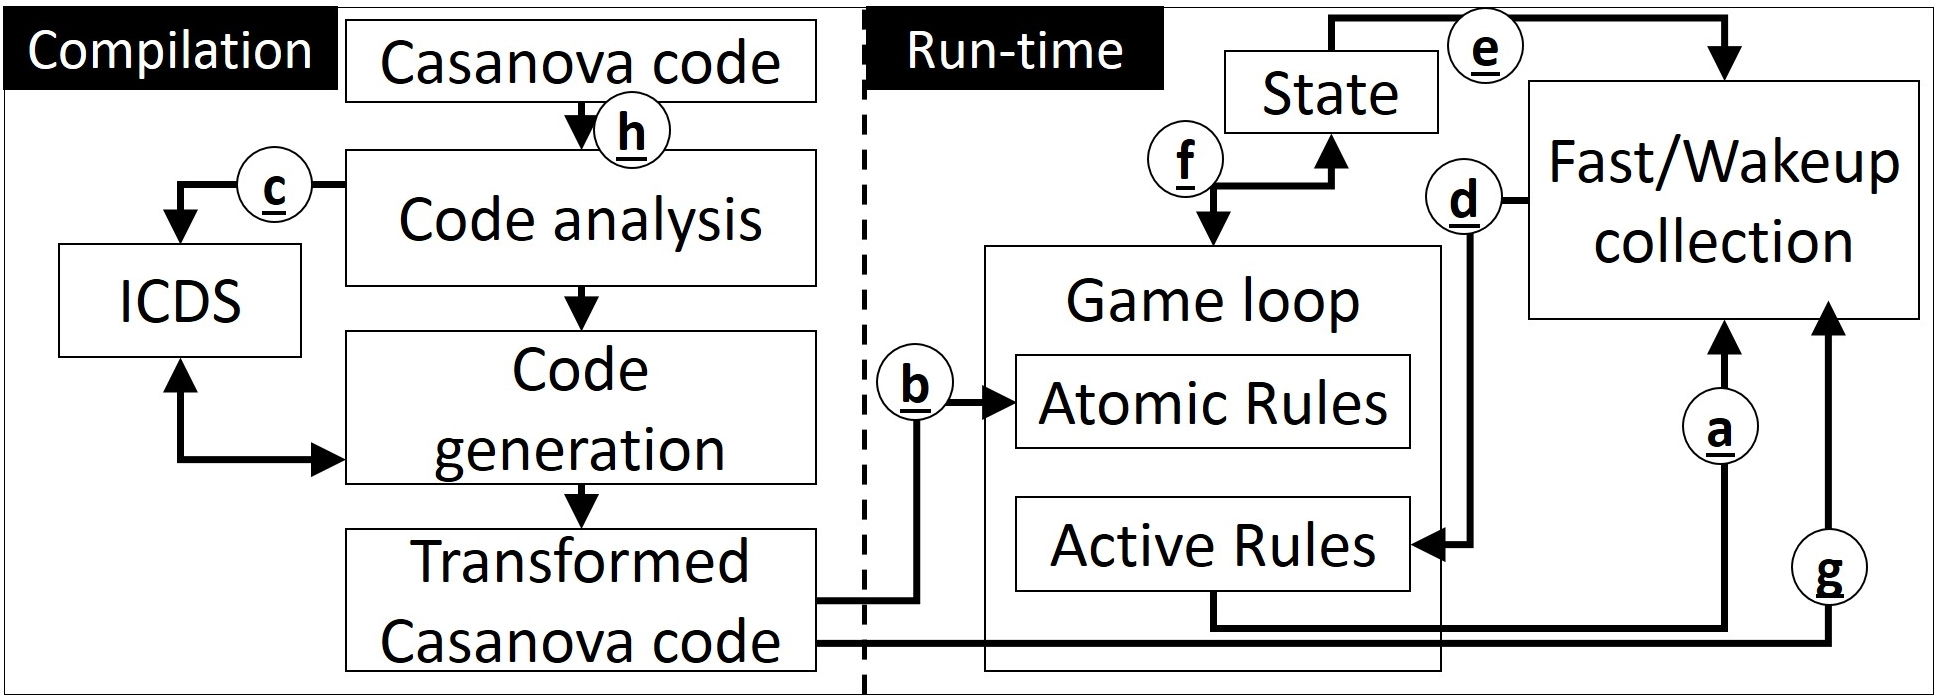
\includegraphics[scale=0.18]{Figures/system_description.jpg}
         \caption{System Configuration}
         \label{fig:system_configuration}
\end{figure}
\vspace{-10pt}


\paragraph*{Casanova overview}
Casanova is a \textit{Domain Specific Language} oriented towards game development. A program in Casanova is a set of entities organized in a tree hierarchy, of which the root is marked as \textit{world}. Each entity contains a set of fields, a set of rules, and a constructor. An extensive description of the formal grammar and semantics of Casanova can be found in \cite{maggiore2013casanova}. Casanova 2 (which we use) is a recent iteration of the original Casanova, which does not introduce changes to syntax or semantics.

In Casanova the state of a game changes only upon the execution of a \textit{rule}. A rule is a block of code acting on a subset of the entity fields called \textit{domain}, which has at least one \texttt{yield} statement and zero or more \texttt{wait} statements. The former updates the value of the fields of an entity, the latter suspends the evaluation of the rule until its condition is met, temporally affecting the fields update. The rule body is re-executed once the end is reached.

An example of a rule that illustrates the \texttt{wait} statement (which specifies that a shield is repaired when it gets damaged) is the following :
\begin{lstlisting}
rule Shields = wait Shields < 0; ...; yield Shields + 1
\end{lstlisting}
\paragraph*{Compilation - Recognizing ICs in Casanova}
From here on we will refer to the \texttt{wait} predicate as an IC, since its value affects the update of an entity with respect to the flow of time.

We also include query conditions in our IC taxonomy. We can think of a query as an entity containing a list of valid query elements that satisfy the \texttt{where} condition. An element adds itself to the valid query elements only if it satisfies the query \texttt{where} condition (this is done by adding to its rules a rule that starts with a \texttt{wait} on the query condition and ends with a \texttt{yield} that appends itself to the valid query elements).

An example of a rule with a query (which selects ships that are not destroyed) is the following:
\begin{lstlisting}
rule Ships = yield from s in Ships do
                   where s.Life > 0
                   select s
\end{lstlisting}
The effect of a \texttt{yield} is to suspend the execution of the rule for one frame and to assign the selected query elements to the selected field. To achieve the optimization as described in the previous section, the compiler uses an optimization analyzer (composed by a code analyzer and a code generator as shown in Figure \ref{fig:system_configuration}(h)), which requires the identification of ICs in code. This is discussed next.

Casanova allows interaction with external libraries and frameworks such as the .NET framework. Because the analyzer cannot infer the temporal behavior of external libraries, we add the restriction that an IC must be fully dependent on Casanova data types. The restriction is necessary because the analysis will lead to alterations in the structure of the game code and field creation, update, and access.

Given the informal considerations above, we introduce the following definitions:
\begin{inparaenum}[i)]
\item A \textit{suspendable statement} is either a \texttt{wait} or a \texttt{yield};
\item a \textit{suspendable rule} is a rule containing a suspendable statement. A suspendable rule is \textit{interesting} (ISR) if the \texttt{wait} argument is an IC or a \texttt{yield} on a query.
\item An \textit{atomic rule} is a rule which does not contain suspendable statements.
\end{inparaenum}

We now present two algorithms that respectively check if a predicate is affected by an atomic rule (Algorithm \ref{alg:atomic}) and to build the ICDS (Algorithm \ref{alg:icds_construction}). For brevity we do not present the procedure to check if a rule is an ISR, which can be done by simply looking at the syntax tree of the rule body.

\vspace{-5pt}
\begin{algorithm}
\caption{Check if a predicate is affected by an atomic rule}
\tiny
\label{alg:atomic}
\begin{algorithmic}
\Function{Atomic}{$p$}
    \State $E$ is the set of entities.
    \State $DFA \gets \emptyset$

    \For {$e \in E$}
        \State $R$ is the set of rules in $e$
        \For {$r \in R$}
            \If {$r$ is an atomic rule}
                \For{$f \in r.domain$}
                    \State $DFA \cup \lbrace (e,f) \rbrace$
                \EndFor
            \EndIf
        \EndFor
    \EndFor
    \State $D \gets$ set of $(entity,field)$ in the predicate $p$.
    \State \Return $\exists x \in D \; : \; x \in DFA$.
\EndFunction
\end{algorithmic}
\end{algorithm}
\vspace{-22pt}
\begin{algorithm}
\caption{ICDS construction}
\tiny
\label{alg:icds_construction}
\begin{algorithmic}
\Function{buildICDS}{ }
    \State $ICDS \gets \emptyset$
    \State $E$ is the set of entities.

    \For {$e \in E$}
        \State $R$ is the set of rules in $e$
        \For {$r \in R$}
            \If {$r$ is an ISR}
                \State $p$ is the first interesting condition of $r$
                \If {\textbf{not} \Call{Atomic}{$p$}}
                    \State $ICDS \cup \lbrace (e,r.index,r.domain,p) \rbrace$
                \EndIf
            \EndIf
        \EndFor
    \EndFor
    \State \Return $ICDS$
\EndFunction
\end{algorithmic}
\end{algorithm}
\vspace{-5pt}

Given a Casanova program, we build the ICDS data structure as follows: we iterate over every entity; for every rule in each entity, if the rule is suspendable, interesting and the predicate does not contain fields that are affected by an atomic rule, we add the entity, the rule index, the rule domain, and the predicate to the ICDS (See Figure \ref{fig:system_configuration}(c)).

We now focus on the identification of interesting conditions that exhibit temporal locality.

\paragraph*{Run-time efficient sleep/wake-up system}

We use the data structure generated by the analyzer to produce two distinct kinds of rules: atomic rules (see Figure \ref{fig:system_configuration}(b)) that are run every frame, and suspendable rules (see Figure \ref{fig:system_configuration}(g)). Every suspendable rule depends on an IC. %In the next section we discuss how to deal with those rules to gain higher performance.
%An idea to automatically identify entities that exhibit temporal locality is done by means of exponential regression on game entities data behavior (such as the data presented above).
Because of the property of temporal locality of rules that contain ICs, they do not need to run at every frame. Therefore the game program should activate and deactivate rules as needed at run time. The game needs to: (\textit{i}) activate a suspendable rule when its IC changes value, and (\textit{ii}) deactivate a suspendable rule when its IC is not satisfied (i.e., when it is \texttt{false}). The game keeps a rule active as long as the evaluation of its IC is \texttt{true}. Suspendable rules differ from classic atomic rules in Casanova since suspendable rules may become inactive, i.e., they do not run during every update in the game loop.

We define the \emph{Object Set} (\texttt{OBS}) as the set of pairs made of an instance of an entity and its field, that appear as arguments in an IC. Information used to build an \texttt{OBS} is collected by using the ICDS. The idea behind the optimization is that, whenever the field of an element of \texttt{OBS} changes during the game loop (see Figure \ref{fig:system_configuration}(f)), we activate the corresponding \emph{Interesting Suspendable Rule} (ISR) \texttt{R} by triggering it (see Figure \ref{fig:system_configuration}(e)).

\vspace{-0.056in}
We implement the previous behavior by means of dictionaries that keep track of the dependencies among \texttt{OBS} and \texttt{R}. We use dictionaries in this implementation since they exhibit the best asymptotic complexity with respect to the following operations: check, add, remove, and iterate. From now on we will refer these dictionaries as \emph{Dictionary of Entity-Predicate} \texttt{DEP}.

We use the static information from the ICDS (see Figure \ref{fig:system_configuration}(c)) to refer to the appropriate dictionary, based on the shape of the IC, to generate unique names for dictionaries. For every field in the predicate, we combine the name of the type of the object containing the field, the name of the field itself, the entity containing the ISR, and the ISR index.

As key we use a pair made of the reference to the object containing the field of the IC and the field itself. As value we store a collection of pairs made of the instance of the entity containing the ISR and the ISR index. We use a collection because it might be the case that one or more instances of the same entity type are pending on the same specific object field. In the example below the rule in \texttt{E} waits on a field \texttt{X} in the \texttt{world}, and the \texttt{world} contains a collection of instances of \texttt{E}. When \texttt{X} changes, all the rules of each instance of \texttt{E} waiting for \texttt{X} must be resumed.

\begin{lstlisting}
world W = X : int; L : List<E>
          rule X = wait 10; yield X + 1
          ...
entity E = ...
           rule Y = wait world.X % 2 = 0; ...
\end{lstlisting}

An entry of the dictionary in the example would be \texttt{(world,X), (L[0],rule Y)}.

\paragraph*{Suspendable rules instantiate, destroy, and update}

In order to maintain the suspendable rules we identify three stages that represent the life cycle of a suspendable rule:
\begin{inparaenum}[i)]
\item \textbf{On creation}: when we instantiate an element of which a field appears in one of the pairs of \texttt{OBS}, we use the instance and the field itself as a key to populate all its DEPs with an empty collection as value. When we instantiate an entity of which rules are targeted by an IC, we add the pair made of the entity instance and each targeted rule as a value in its DEPs;
\item \textbf{On destroy}: when an instance which appears either as a value or a key in one of DEPs, we remove all the occurrences of the instance in DEPs;
\item \textbf{On update}: when a field of an IC changes we notify the entities pending on it. After generating the IC data structure, we can safely refer to the dictionaries relying on the fact that the generated code is sound and will not produce errors at run-time. As a consequence of a notification, the ISRs involved in the notification will be activated during the next frame (if they were inactive). We add them to a collection representing the active rules of the entity containing the involved ISRs (see Figure \ref{fig:system_configuration}(d)). We group instances of the same target type into the same collection to achieve better performance (we iterate the active rules all at the same time per type instead of iterating them while iterating each entity). We store a collection in the world that contains per entity all the suspended rules that are run during a game iteration.
\end{inparaenum}


Rules in Casanova are translated at compile time into a series of switches without nesting within functions which return \texttt{void}. ISRs return \texttt{Done} when the evaluation of their IC is \texttt{false} (stay inactive) or \texttt{Working} when the evaluation of their IC is \texttt{true} (go active) or we are still busy with the execution of the block after the IC. When a suspendable rule gets suspended, i.e., its evaluation returns \texttt{Done}, we simply remove it from the active rules collection (see Figure \ref{fig:system_configuration}(a)).

\paragraph*{Query interpretation}


We transform a query into semantically equivalent code where every entity appearing in the \texttt{from} expression (\textit{source}) adds or removes itself from an index stored in the entity containing the query (\textit{target}). We add or remove a source entity in the target index only if the condition is \texttt{true}. This is done by generating a rule that waits for the condition to be \texttt{true} in the target entity. Applying our optimization to queries means that we do not need to iterate conditions every frame: we keep the rule suspended until the condition changes its value.

\begin{comment}
\paragraph*{Examples}

In the following we present three code snippets, and discuss briefly how they are interpreted by the aforementioned approach.

The first snippet below, a suspended rule update, presents the entity \texttt{E}, which contains a rule that waits until the condition \texttt{C} become \texttt{true} and a rule that updates \texttt{C} every five seconds. \texttt{C} is an interesting condition and changes only occasionally, thus the associated rule, which updates F, can benefit from optimization.
\begin{lstlisting}[frame=tlrb]{Name}
entity E =
    F  : T
    C  : bool
    rule F =
        wait C
        B
    rule C =
        wait 5.0f
        yield not C
\end{lstlisting}

The second snippet, an atomic rule update, behaves similarly to the previous one, except that \texttt{C} changes every frame. In this case \texttt{C} is an interesting condition, but the rule that changes \texttt{F} will not benefit from the optimization as \texttt{C} changes constantly.
\begin{lstlisting}[frame=tlrb]{Name}
entity E =
    F  : T
    C  : bool
    rule F =
        wait C
        B
    rule C = yield not C
\end{lstlisting}

In the third snippet, a suspended query rule update, \texttt{F} is updated by selecting those elements in \texttt{Elems} (a collection of elements of type \texttt{S}) that satisfy a condition \texttt{C}. \texttt{C} is a field in \texttt{S} which changes every five seconds.
\begin{lstlisting}[frame=tlrb]{Name}
entity E =
    F     : [T]
    Elems : [S]
    rule F =
        [for e in Elems do
         where e.C
         select e]

entity S =
    C : bool
    rule C =
        wait 5.0f
        yield not C
\end{lstlisting}

[PS: THE NEXT SENTENCE STILL DOES NOT MAKE SENSE]
Our semantics interpret the third snippet above so that to update the field \texttt{Elems}\texttt{E} only when a condition \texttt{C} is updated. We delegate the evaluation of the condition \texttt{C} to \texttt{S} so to benefit from the optimization as follows:
\begin{lstlisting}
entity E =
    F     : [T]
    Elems : [S]

entity S =
    ref SourceE : E
    C     : bool
    rule SourceE.F =
        wait C
        yield this @ SourceE.F
\end{lstlisting}
\end{comment}
% In the next section we discuss the evaluation in terms of performance and code length of our system. 